
\begin{figure}
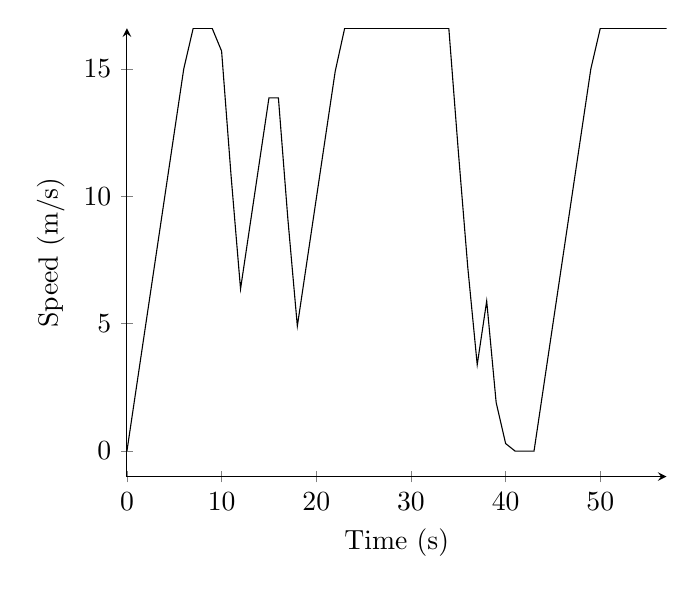
\begin{tikzpicture}
\begin{axis}[
legend style={anchor=west},
axis x line=bottom,
axis y line=left,
ymin=-1,
xlabel=Time (s),
ylabel=Speed (m/s),
]
\addplot[] coordinates {
(0, 0.0)
(1, 2.5)
(2, 5.0)
(3, 7.5)
(4, 10.0)
(5, 12.5)
(6, 15.0)
(7, 16.6)
(8, 16.6)
(9, 16.6)
(10, 15.7025344142)
(11, 10.8098062758)
(12, 6.36332931374)
(13, 8.86332931374)
(14, 11.3633293137)
(15, 13.8633293137)
(16, 13.8678661325)
(17, 9.11018567292)
(18, 4.90850507609)
(19, 7.40850507609)
(20, 9.90850507609)
(21, 12.4085050761)
(22, 14.9085050761)
(23, 16.6)
(24, 16.6)
(25, 16.6)
(26, 16.6)
(27, 16.6)
(28, 16.6)
(29, 16.6)
(30, 16.6)
(31, 16.6)
(32, 16.6)
(33, 16.6)
(34, 16.6)
(35, 11.7832836796)
(36, 7.22292608595)
(37, 3.38992338856)
(38, 5.88992338856)
(39, 1.90521978933)
(40, 0.295225368932)
(41, 0.0)
(42, 0.0)
(43, 0.0)
(44, 2.5)
(45, 5.0)
(46, 7.5)
(47, 10.0)
(48, 12.5)
(49, 15.0)
(50, 16.6)
(51, 16.6)
(52, 16.6)
(53, 16.6)
(54, 16.6)
(55, 16.6)
(56, 16.6)
(57, 16.6)
};

\end{axis}
\end{tikzpicture}
\label{tik:100:8}
\caption{100 percent diving with GSC on route $8$}
\end{figure}
